\documentclass[titlepage,12pt]{article}


\usepackage[utf8]{inputenc}
\usepackage[spanish]{babel}
\usepackage{cancel}
\usepackage{graphicx}
\usepackage{subfig}
\usepackage{caption}
\usepackage{lipsum}
\usepackage{mathtools}
\usepackage{amsmath}
\usepackage{amssymb}
\usepackage{xcolor}
\usepackage[colorlinks=true,urlcolor=blue,linkcolor=black,citecolor=red]{hyperref}
\usepackage[a4paper,margin=2cm]{geometry}


\numberwithin{equation}{section}
\setlength{\parindent}{0.8cm}

\title{\textbf{Almacenamiento de memoria y transiciones de fase en una red de Hopfield}}
\author{}
\date{\today}

\begin{document}
	\maketitle
	\fontsize{15pt}{0}\tableofcontents
	\newpage
	
	
	\section{Red de Hopfield}
	\fontsize{12pt}{0}
	La red de Hopfield es un modelo de red neuronal propuesto por Hopfield en 1982 \cite{hopfield82}. Se trata de una red formada por $N$ neuronas, las cuales sólo pueden tener dos estados: $\sigma_i = +1$ (``encendido'') o $\sigma_i=-1$ (``apagado''), los cuales evolucionan en el tiempo, de forma discreta con pasos temporales finitos $\Delta t$. Estas neuronas interaccionarán entre sí con pesos $J_{ij}$, de modo que el potencial sobre una de las neuronas debido a su interacción con las demás es:
	\begin{displaymath}
	\Phi_i(t)=\sum_{j\neq i} J_{ij}\sigma_j
	\end{displaymath}
	El fin de estas redes es el almacenamiento y la reproducción de patrones. Podemos definir un patrón $\mu$ como una configuración dada de la red, $\mathcal{P}^\mu_i = \pm1, i \in[1,N]$. Entonces, considerando que la evolución de los estados neuronales se da en pasos temporales finitos $\Delta t$, la red habrá reproducido correctamente el patrón $\mu$ si $\sigma_i(t)=\sigma_i(t+\Delta t)=\mathcal{P}^\mu_i$; o dicho de otro modo, los patrones deberán ser puntos fijos de la dinámica. En general, consideraremos que la red almacena un número $K$ de patrones, de modo que $\mu\in[1,K]$. También consideraremos que los patrones sean ortogonales, de modo que:
	\begin{equation}
	\frac{1}{N}\sum_{i=1}^N \mathcal{P}^\mu_i \mathcal{P}^\nu_i = \delta^{\mu\nu}
	\label{ortpat}
	\end{equation}
	\subsection{Analogía con sistemas magnéticos. Hamiltoniano de Ising}
	Este modelo es muy similar al modelo de Ising para un sistema magnético. Acogiéndonos a esta analogía, bajo la restricción de simetría en las interacciones ($J_{ij}=J_{ji}$), podemos utilizar el hamiltoniano del modelo de Ising (a campo magnético $\vec{B}=0$, situación para la que se puede observar la transición ferromagnético-paramagnético) para la dinámica de un sistema de espines $\sigma_i$ a una temperatura $T$, para describir la dinámica de nuestra red de Hopfield.
	\begin{equation}
	H = \frac{1}{2}\sum_{i}\sum_{j\neq i}J_{ij}\sigma_i\sigma_j
	\label{HIsing}
	\end{equation}
	dada la utilidad de esta analogía, por comodidad y abusando del lenguaje, llamaremos ``espines'' a los estados de las neuronas $\sigma_i$ que hemos definido anteriormente. 

	Podemos cuantificar la similitud entre el estado en el que se encuentra la red $\sigma_i$ y el patrón que buscamos reproducir $\mathcal{P}^\mu_i$ definiendo el solapamiento:
	\begin{equation}
	m^\mu(t)=\frac{1}{N}\sum_i \mathcal{P}^\mu_i\sigma_i(t)
	\label{overlap}
	\end{equation}
	que toma el valor máximo $m^\mu = 1$ cuando la red reproduce exactamente el patrón, es decir, $\sigma_i = \mathcal{P}^\mu_i\hspace{0.2cm}\forall i$.
	
	Estos estados estacionarios vienen determinados por la forma de los pesos de la interacción $J_{ij}$, es decir, son los responsables del almacenamiento de los patrones $\mathcal{P}^\mu_i$. Recordemos que hemos elegido el caso simétrico, $J_{ij}=J_{ji}$. Estos pesos pueden interpretarse como elementos de una matriz. Si queremos que nuestra red sea capaz de reproducir (recordar) un número $K$ de patrones $\mathcal{P}^\mu_i$ previamente almacenados, buscamos que los $J_{ij}$ establezcan una correlación entre los estados y el patrón. Para ello, la forma más simple que pueden tomar es:
	\begin{equation}
	J_{ij}=\frac{1}{N}\sum_{\mu=1}^K \mathcal{P}^\mu_i \mathcal{P}^\mu_j
	\label{Jint}
	\end{equation}
	dónde $N$ es el número de neuronas (o espines) en la red; en el límite termodinámico (LT), $N\rightarrow\infty$ mientras que para una red finita $D$-dimensional de lado $L$, $N=L^D$. Recordemos que $\mathcal{P}^\mu_i = \pm1$, y que los patrones ortogonales de modo que los $\mathcal{P}^\mu_i$ satisfacen \eqref{ortpat}.
	\section{Generalización del modelo de Hopfield}
	Hasta ahora hemos visto que la red de Hopfield admite ser interpretada como un modelo de Ising, por su analogía con un sistema magnético de espines que sólo pueden tener dos orientaciones posibles. Además, la red de Hopfield sigue una dinámica dónde, empezando desde una configuración arbitraria, el sistema evoluciona a través de una secuencia de cambios de espín (que involucra aquellos espines desalineados con sus campos moleculares). En esencia, esta es una dinámica de Monte Carlo o Glauber, dónde el proceso produce un decrecimiento monótono del hamiltoniano \eqref{HIsing}, es decir, disminuye la energía. Sin embargo, hasta ahora hemos tratado un sistema sin ruido; en un sistema con ruido se pueden llegar a configuraciones fuera de la dinámica que estamos tratando. Para solventar este problema, se introduce una temperatura efectiva $T$ que caracteriza el nivel de ruido en el sistema \cite{amit1}. La generalización natural del modelo a un sistema con dicho ruido es adoptar la dinámica de espines de Glauber a una temperatura finita $T$, dónde la distribución de las configuraciones se relaja a una distribución de Gibbs.
	\begin{displaymath}
	P(\lbrace\sigma\rbrace)\propto e^{-H(\lbrace\sigma\rbrace)/T}
	\end{displaymath}
	Este modelo se conoce como el modelo de Hopfield generalizado. En este nuevo caso, la estabilidad de un estado a todos los cambios de espín individuales no es suficiente para la estabilidad dinámica a temperaturas finitas. 
	\subsection{Teoría de campo medio para el modelo}
	Ahora, estudiemos el hamiltoniano \eqref{HIsing} con los pesos de interacción \eqref{Jint}, para un número de patrones o memorias $K$ finito. Posteriormente tomaremos el LT, $N\rightarrow\infty$. La densidad de energía libre será:
	\begin{equation}
	f(T)=-\frac{T}{N}\left<\log Z\right>_{\mathcal{P}}
	\label{famit}
	\end{equation}
	dónde $\left<\cdot\right>_\mathcal{P}$ es el promedio sobre la distribución de patrones $\lbrace\mathcal{P}^\mu_i\rbrace$ y $Z$ es la función de partición.
	\begin{equation}
	Z=\sum_{\lbrace\sigma\rbrace}e^{-H(\lbrace\sigma\rbrace)/T}=\left(\frac{N}{T}\right)^{\frac{K}{2}}e^{-\frac{K}{2T}}\int\prod_\mu \frac{dm^\mu}{\sqrt{2\pi}}\exp\Bigg\{-\frac{N\vec{m}^2}{2T}+\sum_i \log\left[2\cosh\left(\frac{\vec{m}\cdot\vec{\mathcal{P}_i}}{T}\right)\right]\Bigg\}
	\label{Zamit}
	\end{equation}
	dónde hemos introducido la cantidad $m^\mu$, y la notación vectorial $\vec{m}$ y $\vec{\mathcal{P}_i}$, cuyas componentes son los $K$ valores de ambas cantidades. $\vec{m}$ será el parámetro de orden. Si $K$ es finito, la integral estará predominada por su valor de punto de silla, con lo que tenemos:
	\begin{equation}
	-\frac{T\ln Z}{N}=\frac{1}{2}\vec{m}^2-\frac{T}{N}\sum_i\ln\left[2\cosh\left(\frac{\vec{m}\cdot\vec{\mathcal{P}_i}}{T}\right)\right]
	\label{saddlepoint}
	\end{equation}
	y el parámetro de orden viene dado por la ecuación $\partial\ln Z/\partial m^\mu$=0.
	\begin{equation}
	\vec{m}=\frac{1}{N}\sum_i \vec{\mathcal{P}_i}\tanh\left(\frac{\vec{m}\cdot\vec{\mathcal{P}_i}}{T}\right)
	\label{eqm}
	\end{equation}
	para $N$ finito el lado derecho de estas ecuaciones depende de la distribución concreta de patrones, pero en el LT las fluctuaciones se suprimen y las cantidades $\ln Z$ y $\vec{m}$ están auto-promediadas; por tanto, las sumas $(1/N)\sum_i$ se convierten en promedios sobre la distribución {$\vec{\mathcal{P}_i}$}, de dónde obtenemos las ecuaciones de campo medio:
	\begin{equation}
	f(T)=\frac{1}{2}\vec{m}^2 - T\left<\log\left[2\cosh\left(\frac{\vec{m}\cdot\vec{\mathcal{P}_i}}{T}\right)\right]\right>_{\mathcal{P}}
	\label{meanfieldf}
	\end{equation}
	\begin{equation}
	\vec{m}=\left<\vec{\mathcal{P}_i}\cdot\tanh\left(\frac{\vec{m}\cdot\vec{\mathcal{P}_i}}{T}\right)\right>_{\mathcal{P}}
	\label{meanfieldm}
	\end{equation}
	si ahora introducimos el promedio térmico de los espines:
	\begin{equation}
	\left<\sigma_i\right>=\tanh\left(\frac{\vec{m}\cdot\vec{\mathcal{P}_i}}{T}\right)
	\label{thermalspin}
	\end{equation}
	introduciendo \eqref{thermalspin} en \eqref{meanfieldm} obtenemos:
	\begin{equation}
	m^\mu=\left<\mathcal{P}^\mu_i{\left<\sigma_i\right>}\right>_{\mathcal{P}}
	\label{meanfieldoverlap}
	\end{equation}
	comparando \eqref{meanfieldoverlap} con \eqref{overlap}, vemos que el parámetro de orden $\vec{m}$ es el solapamiento promedio. De hecho, esta comparación es más fácil con la ecuación \eqref{meanfieldm}, antes de eliminar el sumatorio que también aparece en \eqref{overlap}. Aquí podemos ver una analogía con el modelo de Ising. En él, el parámetro de orden --la magnetización-- para campo medio tiene la siguiente forma:
	\begin{displaymath}
	\tilde{m}=\left<\sigma_i\right>
	\end{displaymath}
	que es similar a la forma que ha tomado nuestro parámetro de orden, el solapamiento, en \eqref{meanfieldoverlap}. Veremos que esta analogía se puede extender más en el siguiente apartado.
	\subsection{Distribución de los patrones. Estados de Mattis}
	Estudiemos ahora la distribución de los estados que conforman los patrones. Cómo ya hemos establecido en la sección 1, un espín $i$ que forma parte del patrón $\mu$ sólo puede tomar dos valores: $\mathcal{P}^\mu_i=+1$ o $\mathcal{P}^\mu_i=-1$. Entonces, sabemos inmediatamente que hay un 50\% de probabilidad de que $\mathcal{P}^\mu_i$ se encuentre en el primer caso, y otro 50\% de que se encuentre en el segundo. Esto nos da directamente la distribución para un único espín del patrón, que matemáticamente podemos escribir cómo:
	\begin{equation}
	p(\mathcal{P}^\mu_i)=\frac{1}{2}\left[\delta(\mathcal{P}^\mu_i + 1) + \delta(\mathcal{P}^\mu_i - 1)\right]
	\label{distpatind}
	\end{equation}
	Con este resultado en mano, podemos escribir la distribución para los K patrones (o lo que es lo mismo, para $\vec{\mathcal{P}_i}$) cómo:
	\begin{equation}
	P(\lbrace\mathcal{P}^\mu_i\rbrace)=\prod_{\mu,i}p(\mathcal{P}^\mu_i)
	\label{distpat}
	\end{equation}
	Ahora, el desarrollo en serie de potencias de $\vec{m}$ de las ecuaciones \eqref{meanfieldf} y \eqref{meanfieldm} es:
	\begin{align}
	f=&-T\log 2 + \frac{1}{2}(1 - \beta)\vec{m}^2 + o(\vec{m}^4) \label{fseries}\\ m^\mu=&\beta m^\mu + \frac{2}{3}\beta^3 (m^\mu)^3 - \beta^3m^\mu\vec{m}^2 + o(\vec{m}^4) \label{mseries}
	\end{align}
	con $\beta\equiv1/T$ (trabajamos en unidades $k_B=1$). Vemos en \eqref{fseries} que para $T=1$, $f=-T\log2$; y despreciando en el término cúbico en $m^\mu$ a la derecha podemos escribir una versión aproximada de \eqref{mseries}:
	\begin{displaymath}
	m^\mu\approx(\beta-\beta^3\vec{m}^2)m^\mu
	\end{displaymath}
	Si evaluamos esta aproximación en $T=1$, o lo que es igual, $\beta=1$, tenemos que la única solución posible es $\vec{m}=0$ (estado ``paramagnético''), que implica de nuevo por la ecuación \eqref{fseries} $f=-T\log2$. Para $T>1$, $\beta<1$, por lo que la aproximación que hemos tomado en \eqref{mseries} tiene mayor validez y por tanto podemos concluir que la única solución sigue siendo $\vec{m}=0$, y $f=-T\log 2$. Alternativamente, podemos argumentar que sí $T >> 1$, $\beta << 1$ y directamente por \eqref{mseries} $m^\mu \approx 0\,\,\forall\mu$, lo que implica $\vec{m}=0$. 
	
	Esta solución se vuelve inestable sin embargo, por debajo de la temperatura crítica $T_c=1$, dónde aparecerán soluciones con $m^\mu$ no nulas. Por ello definiremos la dimensionalidad de $\vec{m}$, $n$: el número de componentes no nulas de $\vec{m}$ para una solución con $T<1$. Estamos ahora observando un comportamiento crítico; sin embargo, esto no debe sorprendernos pues el modelo que estamos utilizando un modelo inspirado en el modelo de Ising, cuyo fin original es describir sistemas magnéticos donde efectivamente hay un comportamiento crítico, la transición ferromagnético-paramagnético. Se puede ver en \eqref{meanfieldm} y \eqref{distpatind} que alterar el orden o cambiar el signo de las $n$ componentes no nulas no altera las soluciones.
	
	Veamos ahora el caso $n=1$. Este caso es especialmente interesante porque nos devolverá las ecuaciones del modelo de Ising para sistemas magnéticos en campo medio. Supongamos $m^1=m\neq0$ y $m^\mu = 0\,\,\forall \mu>1$. Entonces:
	\begin{equation}
	f=\frac{1}{2}m^2 - T\log\left[2\cosh(\beta m)\right]
	\label{fIsinglike}
	\end{equation}
	\begin{equation}
	m=\tanh(\beta m)
	\label{mIsinglike}
	\end{equation}
	Estas soluciones corresponden a un estado dónde:
	\begin{equation}
	\left<\sigma_i\right>=\mathcal{P}_i^1\tanh(\beta m)
	\label{mattisstate}
	\end{equation}
	si introducimos esta solución en \eqref{meanfieldoverlap} tenemos $m=\left<(\mathcal{P}_i^1)^2\tanh(\beta m)\right>_{\mathcal{P}}$. Cómo $\mathcal{P}^\mu_i=\pm 1$, esto se convierte en $m=\left<\tanh(\beta m)\right>_{\mathcal{P}}$ y, por último, al no aparecer los estados de los patrones, el promedio desaparece. Hemos recuperado \eqref{mIsinglike}. 
	
	El estado \eqref{mattisstate} es equivalente termodinámicamente al estado ferromagnético del modelo de Ising. Existen $2K$ estados de este tipo correspondientes a distintas $\mu$ y a distintos signos de las componentes $m^\mu$. Estos estados se denominan estados de Mattis.
	\section{Ecuación de Langevin para la dinámica de los espines}
	En la sección 1, hicimos un breve comentario sobre la dinámica de los espines, donde establecimos que si un estado es parcialmente similar a aquellos que forman el patrón, la dinámica llevará los espines a dichos estados estacionarios. Feigelman et. al. \cite{feigelman86} proponen la ecuación de Langevin que gobierna esta dinámica. 
	
	El primer paso que tomaremos será añadir una modificación al hamiltoniano en forma de un término con un nuevo potencial $V(\sigma_i)$ para cada espín; lo que en realidad nos interesa no es este potencial en sí, si no su derivada, cuyo fin se hará vigente en las ecuaciones del movimiento. Nuestro hamiltoniano es entonces:
	\begin{equation}
	H = \sum_i V(\sigma_i) + \frac{1}{2}\sum_{i}\sum_{j\neq i}J_{ij}\sigma_i\sigma_j
	\label{Hfeigelman}
	\end{equation}
	
	Las ecuaciones de movimiento dadas por \eqref{Hfeigelman} serán equivalentes a las ecuaciones de Langevin para la evolución de los espines $\sigma_i$. Estas son \cite{feigelman86}:
	\begin{equation}
	\frac{\partial\sigma_i}{\partial t} = -\frac{\partial V(\sigma_i)}{\partial\sigma_i} + \sum_j J_{ij}\sigma_j + h_i\sigma_i + \xi_i(t)
	\label{langevin}
	\end{equation}
	En esta dinámica gobernada por \eqref{langevin} los patrones serán estados estables con un rango de atracción en el espacio de configuración, de modo que si un estado inicial $\tilde{\sigma_i}$ es parcialmente similar a uno de los estados estacionarios que $\sigma_i$ conforman el patrón, la dinámica llevará $\tilde{\sigma_i}$ a $\sigma_i$; este es el mecanismo mediante el cual la red recuerda el patrón.\\
	
	Estudiemos ahora los distintos términos de \eqref{langevin}. En estas ecuaciones aparece la derivada del potencial que hemos introducido anteriormente, ${\partial V(\sigma_i)}/{\partial \sigma_i}$. La razón de ser de este término es asegurar que (al menos casi siempre) el valor dado por esta ecuación para los espines sea $\sigma_i=\pm 1$. Una posible elección de este potencial es $V(\sigma_i)=\lambda\left(\sigma_i^2-1\right)^2$. Cuando el potencial toma esta forma, resolver la dinámica nos lleva al resultado:
	\begin{displaymath}
	\sigma_i = \frac{\pm 1}{\sqrt{1-e^{-2\lambda t}}} \xrightarrow[t \rightarrow \infty]{}\pm 1
	\end{displaymath}
	es decir, vemos que en el límite asintótico de tiempos infinitos, los valores de los espines son los esperados, $\pm 1$. Si se utilizan otros potenciales (por ejemplo cuadráticos en vez de cuárticos) se puede comprobar que este comportamiento puede no replicarse, por eso es necesario introducir el potencial para que la dinámica sea coherente con las reglas del modelo. Por otro lado, el parámetro $\lambda$ debe ser positivo; en el caso de que fuera negativo los espines convergerían a $0$, y en el caso de que fuera $\lambda = 0$ (no hay potencial) los valores crecen sin control. Pero también necesitamos que tenga valores grandes respecto a $1$: se puede comprobar que el valor al que convergen los espines para un valor de $\lambda$ dado es:
	\begin{displaymath}
	|\sigma_i|_{estacionario}=\sqrt{1 + \frac{1}{\lambda}}
	\end{displaymath}
	por tanto necesitamos que, como mínimo, $\lambda >> 1$, o preferiblemente $\lambda\rightarrow\infty$. Este hecho cobrará importancia cuando posteriormente llevemos a cabo simulaciones numéricas con la dinámica gobernada por \eqref{langevin}.

    En efecto, si consideramos que los espines han convergido al patrón $\mathcal{P}^\nu_i$, tenemos que $\sigma_i = \sqrt{1 + \frac{1}{\lambda}} \mathcal{P}^\nu_i$. Imponiendo que el estado sea estacionario en \eqref{langevin}, a $T = 0$ obtenemos:

	\begin{equation*}
	\sum_{j=1}^N J_{ij}\sigma_j - \lambda(\sigma_i^2-1)\sigma_i = \sqrt{1 + \frac{1}{\lambda}} \left( \sum_{\mu=1}^K \mathcal{P}^\mu_i \frac{1}{N} \sum_{j=1}^N \mathcal{P}^\mu_j \mathcal{P}^\nu_j  - \mathcal{P}^\mu_i \right) = 0
	\end{equation*} 
	
	Por otro lado, hemos introducido el ruido blanco gaussiano $\xi_i(t)$, que satisface $\left<\xi_i(t)\xi_j(t')\right>=2T\delta_{ij}\delta(t-t')$, dónde $T$ es la temperatura efectiva que se introduce en el modelo de Hopfield generalizado que hemos comentado en la sección 2, como representante del ruido de fondo en el sistema.
	
	Por último, tomaremos como pesos de interacción $J_{ij}$ los definidos en \eqref{Jint}. Son la forma más simple que pueden tomar para reproducir la dinámica deseada. 
	
	En el siguiente apartado utilizaremos esta dinámica para, mediante métodos numéricos, examinar como la red (a una temperatura fija dada $T$) evoluciona hacia un patrón dado externamente desde un estado inicial aleatoriamente desordenado, siguiendo la dinámica dada por \eqref{langevin}. En la figura \ref{ejemplo} se muestra un ejemplo.
	\begin{center}
		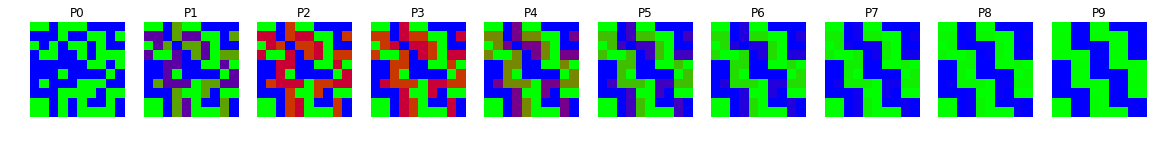
\includegraphics[width=16cm]{pasos.png}
		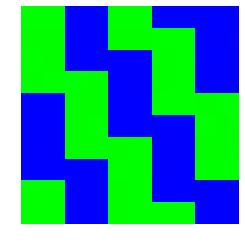
\includegraphics[width=4cm]{final.png} 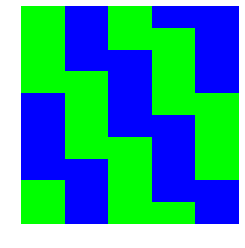
\includegraphics[width=4cm]{patron.png}
		\captionof{figure}{Arriba, la evolución de la red desde el estado desordenado P0 hasta el estado final P9. Abajo, el estado final de la red (izquierda) junto al patrón almacenado (derecha). Vemos que la red ha conseguido reproducir exitosamente el patrón.} \label{ejemplo}
	\end{center}
	\subsection{Simulación numérica de la dinámica}
	En esta sección presentamos una simulación numérica llevada a cabo en Python, utilizando el paquete \verb|neurodynex| proporcionado en \cite{neurodyn-ex}.
	
	Para poder tratar el problema de este modo, el primer paso que hemos de tomar es traducir la ecuación diferencial \eqref{langevin} a una de diferencias finitas. Como ya comentamos en la sección 1, la dinámica de la red neuronal evoluciona por pasos temporales finitos, la dinámica de decaimiento exponencial debe ser rápida (en tiempos de orden $1$), mientras que la dinámica debida al modelo de Ising debe ser lenta.
	\begin{displaymath}
	\sigma_i(t+dt) - \sigma_i(t) = \left(  -4\lambda(\sigma_i^2 - 1)\sigma_i +  \sum_j J_{ij} \sigma_j + h_i\sigma_i \right) dt + \sqrt{2T}dW
	\end{displaymath}
	Absorbiendo el $4$ en el parámetro $\lambda$ y despejando, obtenemos:
	\begin{equation}
	\sigma_i(t+dt) = g(\sigma_i(t)) = \left(  -\lambda(\sigma_i^2 - 1)\sigma_i +  \sum_j J_{ij} \sigma_j + h_i\sigma_i \right) dt + \sqrt{2T}dW + \sigma_i(t)
	\label{dynfunc}
	\end{equation}
	de forma que $g (\sigma_i(t))$ será la función dinámica que utilicemos en el cálculo. Para convertir la ecuación de Langevin en una ecuación diferencial estocástica, hemos introducido el diferencial estocástico $dW$ que cumple:
\begin{equation*}
\mu(dW) = 0, \hspace{10mm} \sigma^2(dW) = dt
\end{equation*}
	\begin{thebibliography}{9}
		\bibitem[1]{hopfield82}{J. J. Hopfield, \textit{Neural networks and physical systems with emergent collective computational abilities}, Proc. Natl. Acad. Sci. USA, \textbf{79}, 2554-2558, abril de 1982.}
		\bibitem[2]{neurodyn}{W. Gerstner, W. M. Kistler, R. Naud, L. Paninski, \textit{Neuronal Dynamics}, Cambridge University Press, 2014, \href{https://neuronaldynamics.epfl.ch/online/index.html}{https://neuronaldynamics.epfl.ch/online/index.html}.}
		\bibitem[3]{feigelman86}{M. V. Feigelman, L. B. Ioffe, \textit{The Statistical Properties of the Hopfield Model of Memory}, Europhys. Lett., \textbf{1} (4), 197-201, febrero de 1986.}
		\bibitem[4]{amit1}{D. J. Amit, H. Gutfreund, H. Sompolinsky, \textit{Spin-glass models of neural networks}, Physical Review A, \textbf{32} (2), 1007-1018, agosto de 1985.}
		\bibitem[5]{amit2}{D. J. Amit, H. Gutfreund, H. Sompolinsky, \textit{Storing Infinite Numbers of Patterns in a Spin-Glass Model of Neural Networks}, Physical Review Letters, \textbf{55} (14), 1530-1533, septiembre de 1985.}
		\bibitem[6]{neurodyn-ex}{W. Gerstner, W. M. Kistler, R. Naud, L. Paninski, \textit{Neuronal Dynamics: Python Exercises}, \href{https://neuronaldynamics-exercises.readthedocs.io/en/latest/index.html}{https://neuronaldynamics-exercises.readthedocs.io/en/latest/index.html}.}
	\end{thebibliography}
\end{document}
